\documentclass[11pt]{beamer}
\usepackage{multicol}
\usepackage{hyperref}
\hypersetup {
    colorlinks=true,
    linkcolor=.,
    urlcolor=red,
}
\usetheme{Warsaw}

%\definecolor{applegreen}{rgb}{0.55, 0.71, 0.0}
%\usecolortheme[named=applegreen]{structure}

\title{Program Analysis - Herbrand Equivalence}
\subtitle{MidTerm BTP Presentation}

\author{Himanshu Rai}
\institute{Indian Institute of Technology, Palakkad}
\date{27/02/2020}

\begin{document}

\begin{frame}
\titlepage
\end{frame}

\begin{frame}{Herbrand Equivalence}
    \begin{itemize}
        \item \textbf{Herbrand Equivalence} is a kind of expression equivalence
        \item Informally, two expressions are \textbf{Herbrand equivalent at a program point} if they have \textbf{syntactically} the same value across all the execution paths from the start of the program to that particular point
        \begin{itemize}
            \item If $Z = X$ then $Z \cong X$
            \item If $Z = X + Y$ then $Z \cong X + Y$
            \item $X \cong Y$ iff $X + Z \cong Y + Z$
            \item $2 + 2 \ncong 4$
        \end{itemize}
        \item The operators are treated as \textbf{uninterpreted functions}
        \begin{itemize}
            \item $X + Y \ncong Y + X$
            \item $X + (Y + Z) \ncong (X + Y) + Z$
        \end{itemize}
    \end{itemize}
\end{frame}

\begin{frame}{Herbrand Equivalence Analysis}
    \begin{itemize}
        \item In \textbf{Herbrand equivalence analysis}, our universe $\mathcal U$ is the set of \textbf{all possible expressions} that can be formed using constants, variables and operators in the program
        \item Then for \textbf{each program point}, we partition $\mathcal U$ such that two expressions belong to the same class iff they are Herbrand equivalent at that point
        \item Finding \textbf{semantic equivalence} of program expressions is \textbf{an undecidable problem} - so usually some \textbf{restricted form of equivalence} is considered - and Herbrand equivalence is one such
    \end{itemize}
\end{frame}

\begin{frame}{Example of Herbrand Equivalence Computation}
    \begin{figure}[!h]
        \centering
        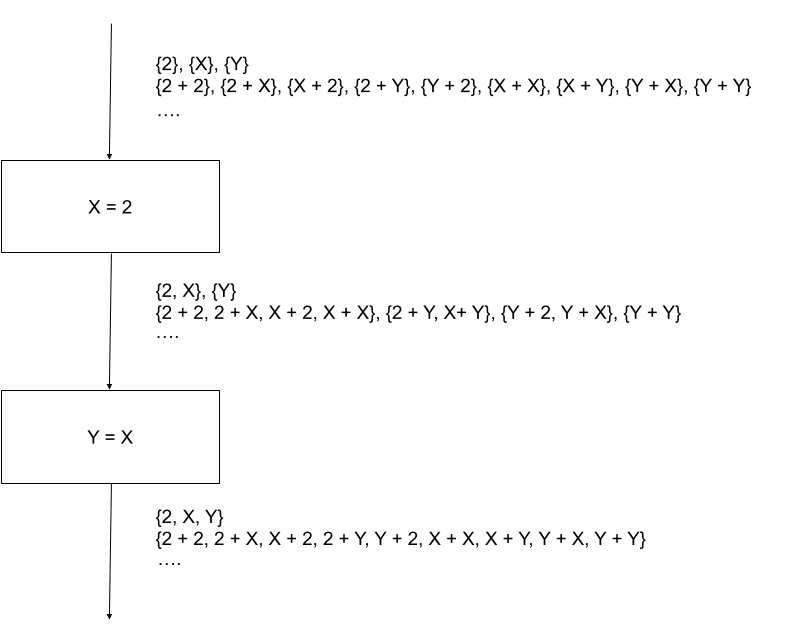
\includegraphics[scale=0.3]{HerbrandEquivalenceTrans.png}
        \caption{Example of Herbrand Equivalence at a \textbf{transfer point}}
        \label{fig:HerbrandEquivalenceTrans}
    \end{figure}
\end{frame}

\begin{frame}{Example of Herbrand Equivalence Computation}
    \begin{figure}[!h]
        \centering
        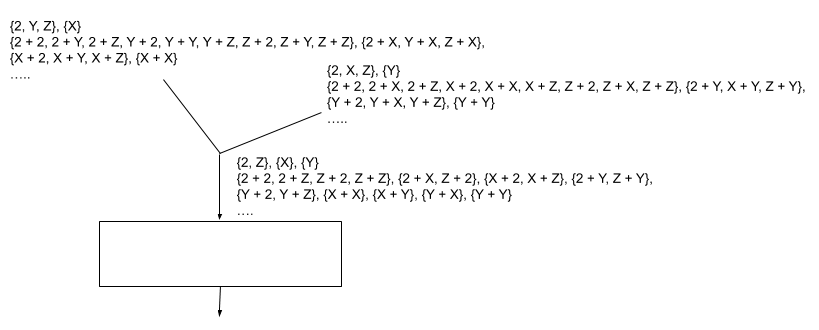
\includegraphics[scale=0.4]{HerbrandEquivalenceConv.png}
        \caption{Example of Herbrand Equivalence at a \textbf{confluence point}}
        \label{fig:HerbrandEquivalenceCon}
    \end{figure}
\end{frame}

\begin{frame}{Idea of the Project}
    \begin{itemize}
        \item Babu, Krishnan and Paleri (in 2019) has given a new lattice theoretic formulation of Herbrand equivalences and proved its equivalence to the classical version
        \item They also gave an algorithm to compute \textbf{Herbrand equivalences associated with program expressions} (expressions that can actually occur in a program)
        \item However, the algorithm does not completely follows the theoretical work, so its correctness/precision needs to be established
    \end{itemize}
\end{frame}

\begin{frame}{Idea of the Project}
    \begin{itemize}
        \item The task of this project is to \textbf{implement the algorithm} for Clang/LLVM compiler framework
        \item Use the equivalence information to \textbf{perform optimizations} and benchmarking it
        \item Also, a \textbf{proof of correctness/precision} of the algorithm has to be presented
    \end{itemize}
\end{frame}

\begin{frame}{Work Done - Last Semester}
    \begin{itemize}
        \item Read few papers related to past works, to get familiarity with the topic
        \item Finished initial implementation of the algorithm for Clang/LLVM compiler framework
    \end{itemize}
\end{frame}

\begin{frame}{Work Done - This Semester}
    \begin{itemize}
        \item Added test cases for verification, corrected errors in the initial implementation
        \item Added Doxygen style comments for proper inline documentation
        \item Expanded code to perform optimizations using analysis information from the earlier implementations
        \item All the codes are available on \href{https://github.com/himanshu520/HerbrandEquivalence}{GitHub} and any further details can be found in the \href{https://github.com/himanshu520/HerbrandEquivalence}{report}
    \end{itemize}
\end{frame}

\begin{frame}{Optimizations done}
    \begin{itemize}
        \item Three kinds of optimizations are done -
        \begin{itemize}
            \item \textbf{Constant propagation} - If $X = 2$, then we can replace all uses of $X$ by $2$
            \item \textbf{Constant folding} - Compute a constant expression at compile time rather than at runtime, eg. $X = 2 + 2$ is same as $X = 4$
            \item \textbf{Redundant expression elimination} - If $X + Y$ is already computed, then we don't need to compute it again
        \end{itemize}
        \item The optimization results are same as those by already existing GVN pass in LLVM, on the test cases it was run
    \end{itemize}
\end{frame}

\begin{frame}{Work in Progress}
    \begin{itemize}
        \item We have already started working on the proof - we realised that modifying the algorithm a bit might be convinient for proving the correctness
        \item We are also parallelly working on getting the benchmarks done
    \end{itemize}
\end{frame}

\begin{frame}{Timeline}
    \begin{itemize}
        \item Adding testcases, verification, improving code, documentation - 2 weeks
        \item Adding optimizations and verifying the results - 2 weeks 
        \item Looking details for benchmarking - 1 week 
        \item New codes and attempt for proof - 3 weeks  
    \end{itemize}
\end{frame}

\end{document}